\chapter{Prerequisiti}
\minitoc

Si pressupone la conoscenza di alcuni concetti fisici di base (la cinematica classica) ed alcuni concetti matematici, 
in particolare è necessario sapere derivare.

\section{La Derivata}

Cominciamo con il ricordare la definizione di derivata:
\begin{Def}[Derivata]
Data una funzione $f(x)$ definita su un intervallo $[a;b]$ a valori reali, si definisce derivata della funzione nel
punto $x=x_0 \in (a;b)$ e si indica con $f'(x_0)$, o con $\dfrac{df}{dx}(x_0)$, il limite  \textit{se esiste finito} del 
rapporto incrementale al tendere a zero dell'incremento $h$, ovvero:
\begin{equation}
 f'(x_0) = \dfrac{\ud f}{\ud x}(x_0) = lim_{h \to 0} \dfrac{f(x_0+h) - f(x_0)}{h}
\end{equation}
\end{Def}

\subsection{Il significato geometrico della derivata}

Perché ci interessa tutto questo? Vedremo che il concetto di derivata viene applicato in fisica per trovare, a partire dalla traiettoria 
di un corpo o, per essere più precisi a partire dalla sua legge oraria\footnote{La legge oraria è una funzione $\ve x(t)$ che restituisce 
la posizione di un corpo in funzione del tempo $t$.}, la velocità e l'accelerazione.

\begin{figure}[htbp]
\centering
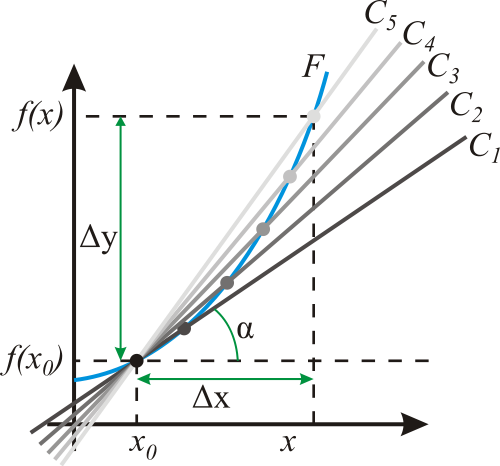
\includegraphics[scale=0.4]{immagini/matematica/derivata}
\caption{\label{img_derivata}Significato geometrico della derivata.}
\end{figure}

Com'è possibile? Dalla definizione (che dovreste ricordare) di velocità cioè:
\begin{equation}\label{mate_velmedia}
 v = \dfrac{s}{t} = \dfrac{\Delta x}{\Delta t}
\end{equation}
abbioamo che, quando l'intervallo di tempo diventa abbastanza piccolo, (ossia quando $\Delta t \to 0$) si ricava:
\begin{equation}
v(t)=\lim_{\Delta t\rightarrow 0} v_m(t,t+\Delta t)=\lim_{\Delta t\rightarrow 0} \frac{\Delta x}{\Delta t}(t)= \left. \frac{\ud x}{\ud t}\right|_t
\end{equation}
dove con $v_m(t, t+ \Delta t)$ indichiamo la velocità media definita come in \ref{mate_velmedia} nell'intervallo $(t, t+\Delta t)$.

Inoltre, come si vede dalla figura \ref{img_derivata}, la derivata, essendo il limite del rapporto incrementale, 
non è nient'altro che il coefficiente angolare della retta tangente alla funzione nel punto $x=x_0$.

Abbiamo quindi che la retta tangente è un ottimo modo per approssimare una funzione in un intorno di un suo punto,
infatti possiamo scrivere:

\begin{equation}\label{first_order}
x(t) \approx x(t_0) + v(t_0)t
\end{equation}

Nel caso di moto rettilineo uniforme la \ref{first_order} è una relazione esatta (non è un'approssimazione).

\subsection{Derivate parziali e derivate direzionali}

Naturalmente la situazione si complica quando si passa da una dimensione, ossia dal moto lungo una retta, descritto da $x(t)$ 
a più dimensioni ($2$ nel piano, $3$ nello spazio), in questo caso possiamo definire la derivata parziale e la derivata 
direzionale: strumenti che generalizzano il concetto di derivata a funzioni di più variabili.

\begin{Def}{Derivata parziale}
Consideriamo una funzione di $n$ variabili $f(\vec{x})= f(x_1, x_2,\ldots,x_n)~:~E\to\mathbb{R}$. Si definisce derivata parziale di $f$ in $\vec{x}\in E$, 
rispetto alla variabile k-esima $x_k$, il limite, se esiste finito, di:
\begin{equation}
    \frac{\partial f(\vec{x})}{\partial x_k}=\lim_{h\to 0}\frac{f(x_1,x_2,\ldots,x_k+h,\ldots,x_n)-f(x_1,x_2,\ldots,x_n)}{h} 
\end{equation} 
\end{Def}

La derivata direzionale di una funzione scalare è la derivata fatta lungo una direzione definita da un vettore (di modulo unitario):
\[ \vec{u} = (u_1, \ldots, u_n) \]
ed è la funzione definita dal limite:
\begin{equation}
D_{\vec{u}}{f}(\vec{x}) = \lim_{h \rightarrow 0^+}{\frac{f(\vec{x} + h\vec{u}) - f(\vec{x})}{h}}.
\end{equation}

\section{Cinematica}

Richiamiamo nel seguito alcuni concetti fondamentali di cinematica: posizione, spostamento, velocità, accelerazione.

\subsection{\index{posizione}Vettore posizione}
\begin{Def}[vettore posizione]
Fissato un sistema di riferimento cartesiano\footnote{per semplicità quasi sempre si parlerà del piano piuttosto che dello spazio, ma i risultati sono del tutto analoghi} 
$xOy$ il vettore che congiunge l'origine con un punto $P$ è il \index{vettore!posizione}vettore posizione $\ve r$ che individua $P$ in quel sistema di riferimento.
\end{Def}

Quindi un punto nello spazio può essere individuato dando tre cordinate $(x_P, y_P, z_P)$, per esempio potete immaginare di dover indicare la 
posizione di un aereo, vi servono latitudine, longitudine, e quota.  È utile a questo punto introdurre i versori.

Poiché un corpo materiale può essere descritto da punto capace di spostarsi nel tempo $\ve r$ sarà funzione del tempo $\ve r=\ve r(t)$ e descriverà al variare del tempo tutte le posizioni occupate da $P$ 
cioè la sua traiettoria\index{traiettoria}.

\begin{figure}[htbp]
\centering
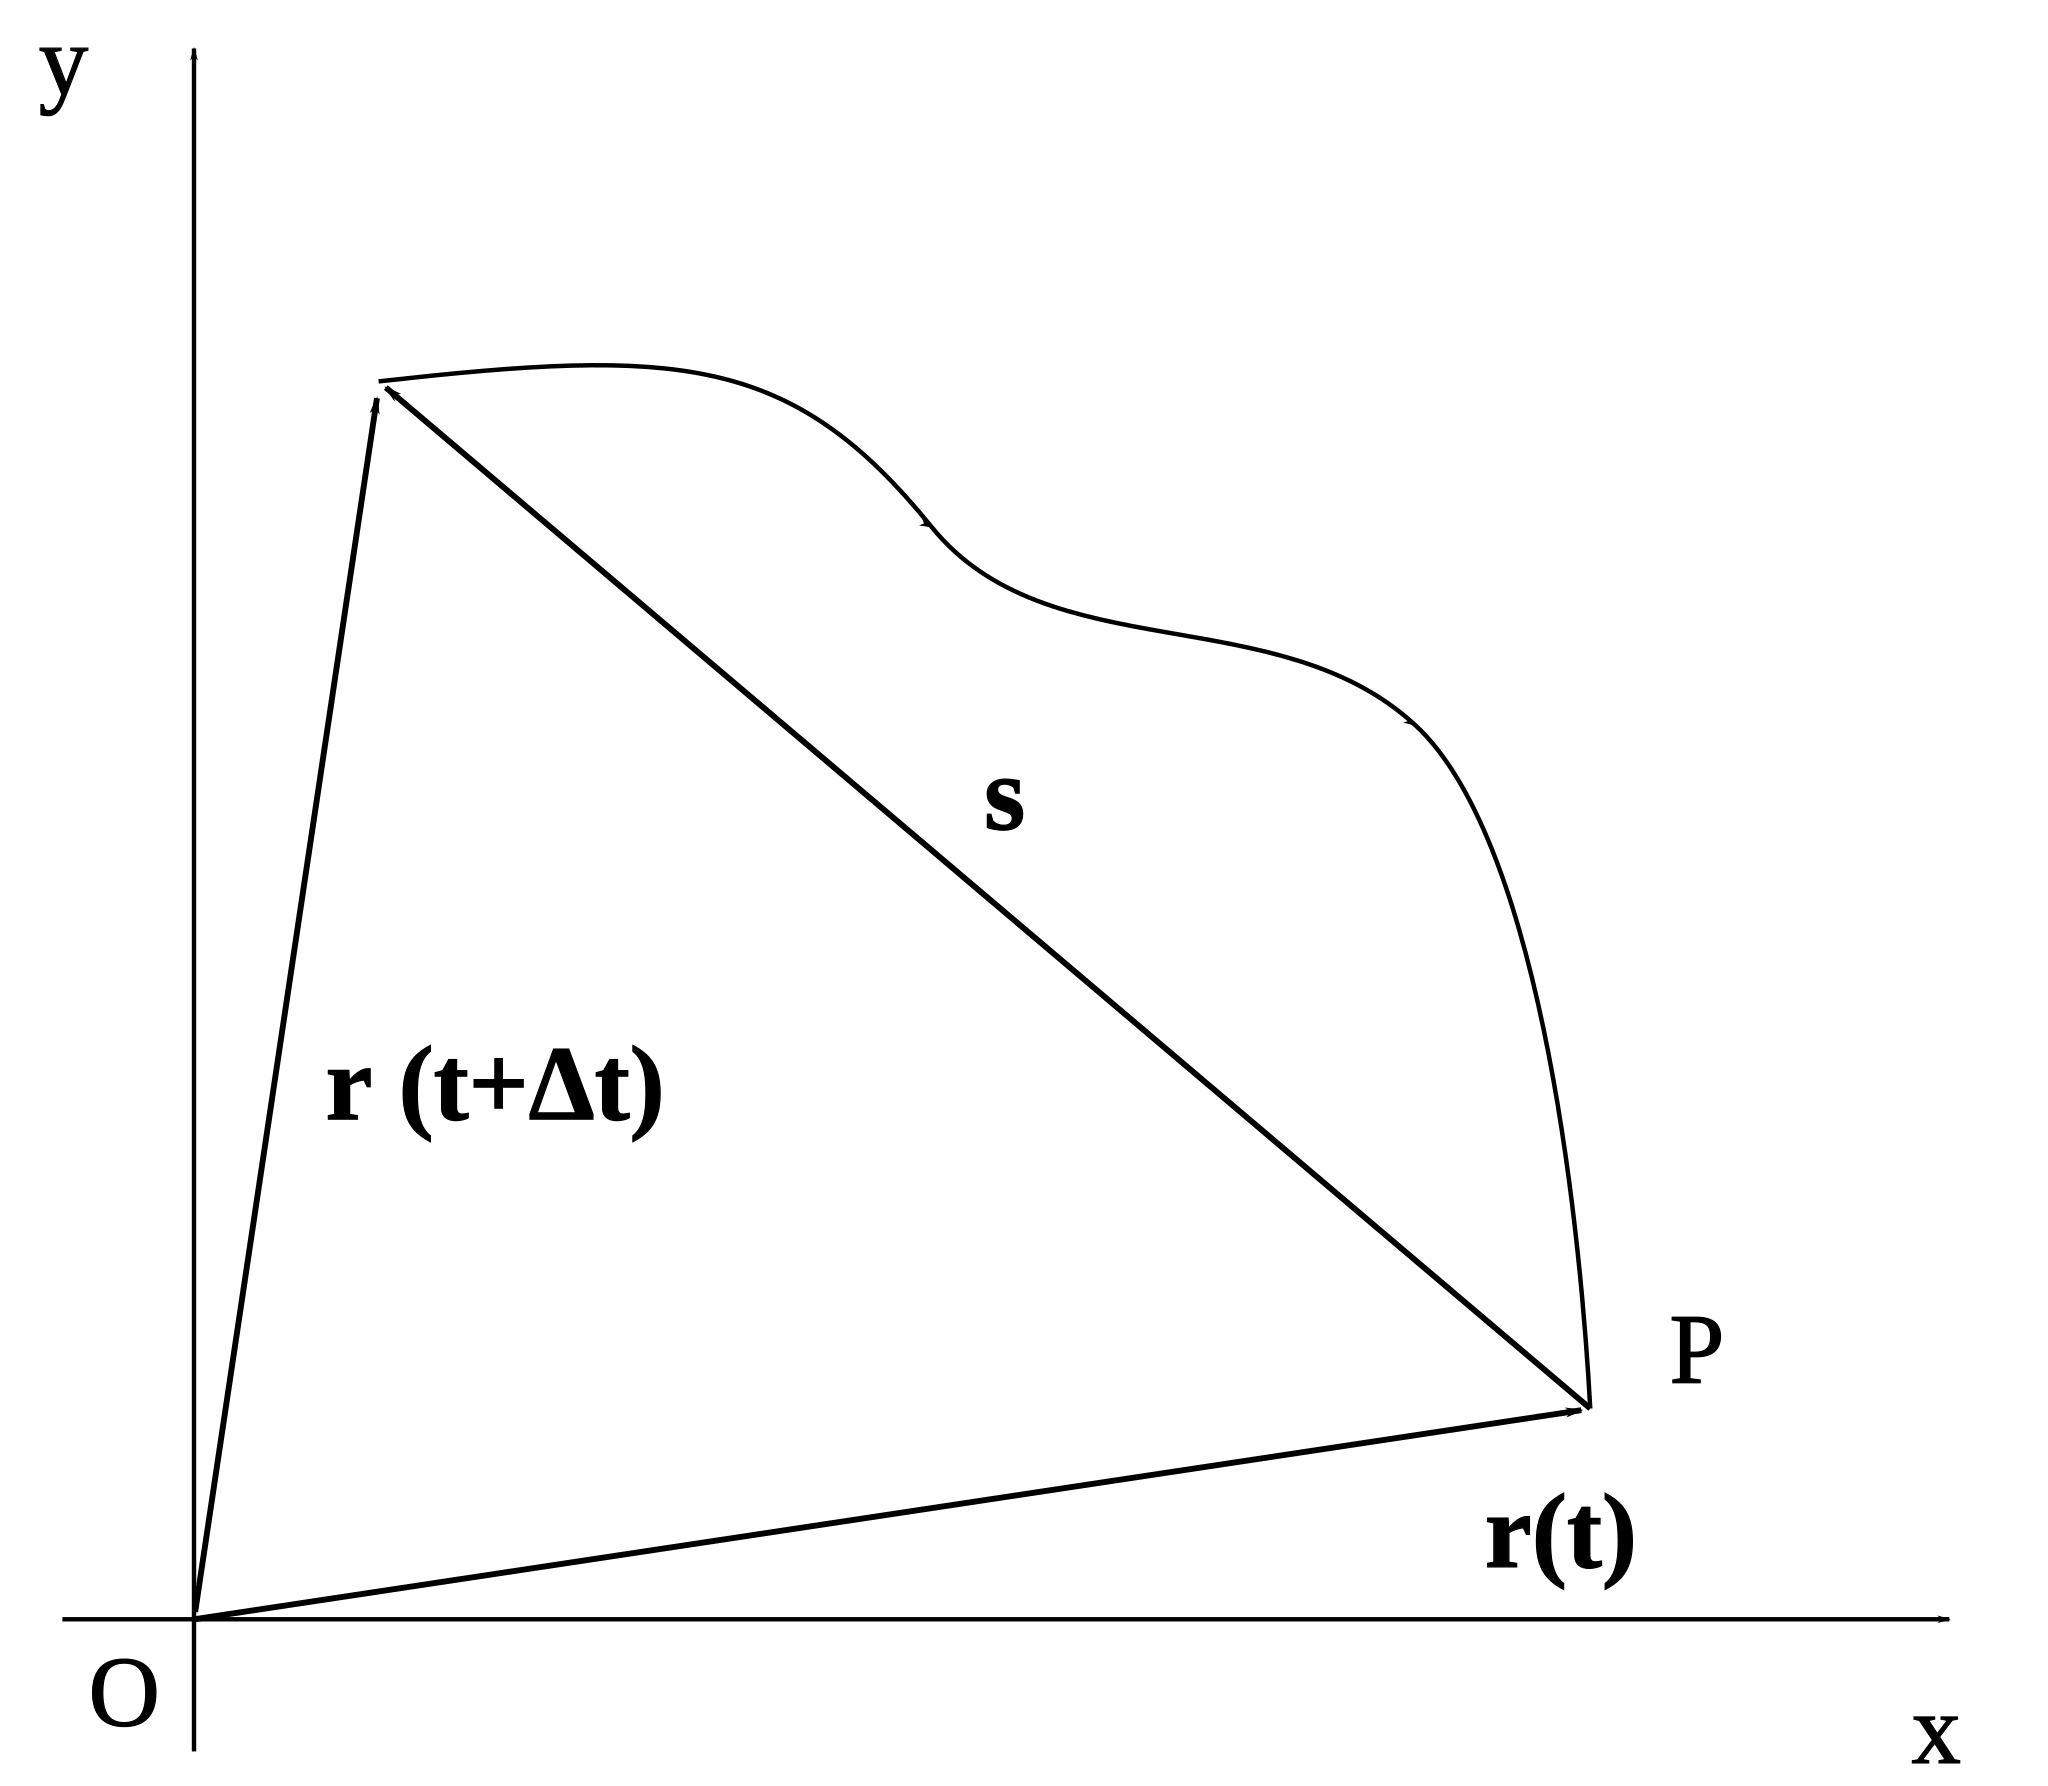
\includegraphics[scale=0.7]{immagini/matematica/vettore_posizione}
\caption{vettore posizione e spostamento.}
\end{figure}

\subsubsection{\index{versore}Versori e \index{coordinate}coordinate}
I versori sono vettori della base ortonormale di $\field{R}^3$ (lo spazio). In parole povere sono sono vettori di modulo unitario 
ortogonali (perpendicolari) a due a due. 
Solitamente si indicano con $\ver i$, $\ver j$ e $\ver k$ i versori applicati nell'origine, nella direzione degli assi cartesiani 
del sistema di riferimento. 

Le loro coordinate sono\footnote{quando si scrive che $\ve v=(a,b,c)$ l'uguaglianza significa che che fissata una base il 
vettore è rappresentato dalle sue coordinate $(a,b,c)$, ma vettori e coordinate non sono la stessa cosa, per esempio 
se si fa un cambiamento di base il vettore non cambia, ma le sue coordinate sì.}:

\begin{equation}
\ver \imath=\left(\begin{array}{c} 1\\0\\0\\ \end{array}\right)\qquad
\ver \jmath=\left(\begin{array}{c} 0\\1\\0\\ \end{array}\right)\qquad
\ver k=\left(\begin{array}{c} 0\\0\\1\\ \end{array}\right)
\end{equation}

Poiché i versori formano una base ogni vettore può essere espresso come una loro combinazione lineare, i coefficienti sono le coordinate\footnote{come già accennato i due simboli di uguaglianza hanno significati diversi, il primo è una vera uguaglianza, il secondo vuol dire che fissata una base, il vettore è rappresentato da quelle coordinate.}:
\begin{equation}
\ve v=v_x\ve i+v_y\ve j+v_z\ve k=\left(
\begin{array}{c}
v_x\\v_y\\v_z\\
\end{array}\right)
\end{equation}

\subsubsection{\index{prodotto!scalare}Prodotto scalare}
Il prodotto scalare usato in fisica è il prodotto scalare canonico della geometria in $\field{R}^3$ rispetto alla base canonica 
$\{\ver i,\ver j,\ver k\}$:

\begin{equation}\label{prodotto_scalare}
\left(\ve{x},\ve{y}\right)=\ve{x}^T\cdot\ve{y}=(x_1y_1+x_2y_2+x_3y_3)
\end{equation}

Un altro modo per esprimerlo è:
\begin{equation}
p_s=|\ve a||\ve b| \cos \alpha
\end{equation}
con $\alpha$ l'angolo compreso tra i due vettori. Da qui si deduce che $\ver i \cdot \ver i=1$, $\ver i
\cdot \ver j=0$, ecc., che due vettori ortogonali hanno prodotto scalare nullo e che due vettori hanno 
prodotto scalare massimo quando sono paralleli.

\[p_s=\ve a \cdot \ve b=(a_x\ve i+a_y\ve j+a_z\ve k)\cdot(b_x\ve
i+b_y\ve j+b_z\ve k)=a_xb_x+a_yb_y+a_zb_z\]

In particolare il prodotto scalare può essere usato per definire la norma\index{norma} (o modulo) di un vettore:
\begin{equation}
||\ve a|| = \sqrt{\ve a \cdot \ve a} = \sqrt{(a_x)^2 + (a_y)^2 + (a_z)^2}
\end{equation}
fatto questo si definisce la distanza\index{distanza} tra due punti nel seguente modo:
\begin{equation}
d(\ve x, \ve y) = ||\ve x - \ve y||
\end{equation}

\subsection{\index{velocità}Vettore velocità}
Applicando la classica definizione:
\begin{equation}\label{vel}
 v = \dfrac{\Delta s}{\Delta t}
\end{equation}
al vettore posizione otteniamo la velocità (vettoriale) media del nostro punto.

\begin{Def}[\index{velocità!media}Velocità Media]
\begin{equation}\label{vel_media}
\ve v_m(t,t+\Delta t)=\frac{\Delta\ve r(t,t+\Delta t)}{\Delta
t}=\frac{1}{\Delta t}\{\Delta x\ve i+\Delta y\ve
j\}=\frac{\Delta x}{\Delta t}\ve i+\frac{\Delta y}{\Delta t}\ve
j 
\end{equation}
\end{Def}

Facendo il limite dell'equazione \ref{vel_media} per $t \to 0$ abbiamo:
\begin{Def}[\index{velocità!istantanea}Velocità Istantanea]
\begin{equation}
\ve v(t)=\lim_{\Delta t\rightarrow 0}\ve v_m(t,t+\Delta t)=\lim_{\Delta t\rightarrow 0} \frac{\Delta\ve r}{\Delta t}(t)={\left.\frac{\ud \ve r}{\ud t}\right|_t}=\left.\frac{\ud x}{\ud t}\right|_t\ve i+\left.\frac{\ud y}{\ud t}\right|_t\ve j
\end{equation}
\end{Def}

\subsection{\index{accelerazione}Vettore accelerazione}
Allo stesso modo possiamo ottenere la definizione di accelerazione istantanea:
\begin{Def}[accelerazione istantanea]
\begin{equation}
 \ve a=\frac{\ud \ve v}{\ud t}={\frac{\ud^2 \ve r}{\ud t^2}}
\end{equation}
\end{Def}

Abbiamo quindi riformulato tutte le definizioni utilizzando il concetto di derivata.

\section[Moto rettilineo uniforme]{\index{moto!rettilineo uniforme}Moto rettilineo uniforme}
Usiamo sempre condizioni iniziali implicite, del tipo $t_0=0$, $\ve r(0)=\ve r_0$, $\ve v(0)=\ve v_0$.
\begin{Def}[moto rettilineo uniforme]
\[\ve v=\overrightarrow\const\]
\end{Def}
\[\ud\ve r=\ve v\,\ud t\qquad\int_{\ve r_0}^{\ve r}\ud\ve r=\int_0^t\ve v\,\ud t \qquad \ve r-\ve r_0=\ve v t\]
\begin{eqimp}{equation}
\ve r=\ve v t+\ve r_0
\end{eqimp}
\section{\index{moto!uniformemente accelerato}Moto uniformemente accelerato}
\begin{Def}[moto uniformemente accelerato]
\[\ve a=\overrightarrow{\const}\]
\end{Def}
\[\ve a\,\ud t=\ud \ve v\qquad\int_0^t\ve a\,\ud t=\int_{\ve v_0}^{\ve v}\ud \ve v\qquad\ve a t=\ve v-\ve v_0\]
\begin{eqimp}{equation}
\ve v=\ve a t+\ve v_0
\label{vt_01}
\end{eqimp}
\[\ve v=\ve a t+\ve v_0=\frac{\ud \ve r}{\ud t}\]
\[\ud \ve r=\left(\ve a t+\ve v_0\right)\ud t\qquad\int_{\ve r_0}^{\ve r}\ud \ve r=\int_0^t\left(\ve a t+\ve v_0\right)\ud t\qquad\ve r-\ve r_0=\frac{1}{2}\ve a t^2+\ve v_0 t\]
\begin{eqimp}{equation}
\ve r=\frac{1}{2}\ve a t^2+\ve v_0 t+\ve r_0
\label{vt_02}
\end{eqimp}

